
% ===============================================
% ECEV 33400: Stochastic Processes      Fall 2017
% notes.tex
% Template for class notes
% ===============================================

% -----------------------------------------------
% The preamble that follows can be ignored. Go on
% down to the section that says "START HERE" 
% -----------------------------------------------

\documentclass{article}

\usepackage[margin=1in]{geometry} 
\usepackage{amsmath,amsthm,amssymb}
\usepackage[ampersand]{easylist}
\usepackage[sectionbib]{natbib}
\usepackage[colorinlistoftodos,prependcaption,textsize=tiny]{todonotes}

\newcommand{\R}{\mathbb{R}}
\newcommand{\Z}{\mathbb{Z}}
\newcommand{\N}{\mathbb{N}}
\newcommand{\Q}{\mathbb{Q}}
\newcommand{\C}{\mathbb{C}}
\newcommand{\F}{{\mathbb F}}
\newcommand{\Pb}{{\mathbb P}}
\newcommand{\E}{{\mathbb E}}
\newcommand{\Frac}[2]{\left(\frac{#1}{#2}\right)}
\newcommand{\Eval}[2]{\big|_{#1}^{#2}}
\newcommand{\intinf}{\int_{-\infty}^{\infty}}

\newenvironment{theorem}[2][Theorem]{\begin{trivlist}
\item[\hskip \labelsep {\bfseries #1}\hskip \labelsep {\bfseries #2.}]}{\end{trivlist}}
\newenvironment{lemma}[2][Lemma]{\begin{trivlist}
\item[\hskip \labelsep {\bfseries #1}\hskip \labelsep {\bfseries #2.}]}{\end{trivlist}}
\newenvironment{exercise}[2][Exercise]{\begin{trivlist}
\item[\hskip \labelsep {\bfseries #1}\hskip \labelsep {\bfseries #2.}]}{\end{trivlist}}
\newenvironment{problem}[2][Problem]{\begin{trivlist}
\item[\hskip \labelsep {\bfseries #1}\hskip \labelsep {\bfseries #2.}]}{\end{trivlist}}
\newenvironment{question}[2][Question]{\begin{trivlist}
\item[\hskip \labelsep {\bfseries #1}\hskip \labelsep {\bfseries #2.}]}{\end{trivlist}}
\newenvironment{corollary}[2][Corollary]{\begin{trivlist}
\item[\hskip \labelsep {\bfseries #1}\hskip \labelsep {\bfseries #2.}]}{\end{trivlist}}

\newenvironment{solution}{\begin{proof}[Solution]}{\end{proof}}


\begin{document}
% ------------------------------------------ %
%                 START HERE                 %
% ------------------------------------------ %
\title{Complexity Science: \\ An introduction to Stochastic Processes in Continuous Time \\ Master on Computational Biomedical Engineering (UPF)} % Replace X with the appropriate number
\author{David Alonso ({\tt dalonso@ceab.csic.es}) \\ Theoretical and Compuational Ecology ({\tt http://www.theelab.net})} % Replace  "\iffalse X \fi" with your name.
\date{\today} % Don't change this! :( 

\maketitle

% ----------- ADD COMMENT COMMANDS --------------------
\newcommand{\ruby}[1]{\todo[color=green!40]{#1 - Ruby}}
\newcommand{\studentX}[1]{\todo[color=green!40]{#1 - studentX}} % replace studentX with your name. 
\newcommand{\vicente}[1]{\todo[color=purple!40]{#1 - vicente}}
\newcommand{\david}[1]{\todo[color=yellow]{#1 - david}}
% -----------------------------------------------------

% -----------------------------------------------------
% Notes from Class 
% -----------------------------------------------------
\section{Introduction}
These are Alonso's notes for an introductory course on Stochastic Processes in Continuous Time. Our main intention is the presentation of the pieces of theory we will need to formalize one-step stochastic processes with some mathematical rigor. First, we begin with basic concepts and definitions of probability theory. We assume the reader is familiar basic calculus and has been exposed to an introductory course on probability and statistics. Then, we derive the Poisson distribution that results from a counting process as a first simple example of a one-step stochastic process. We derive the so-called master equation in this simple case, and show how to solve it. It follows then a general derivation of the master equation for one-step processes in one dimension, and how to find the probability distribution characterizing the stationary state. Then, through several examples, the essence of the Gillespie algorithm is explained as a way to build exact stochastic simulations. Stochastic processes are often used in science to model uncertainty and variability in data collected from a given system. Therefore, the final sections are intended to show the connection between stochastic models and data through the likelihood function. A final example on colonization and extinction processes in an island emphasizes this point.
\smallskip

As you see, these notes cover most topics in a typical syllabus of an introductory course to one-step stochastic processes in continuous time, the so-called birth-death processes. Some examples may (intentionally) slightly differ from those explained in class. Sometimes I give more details here than I did in class, but not always. You can also explore some methods explained here and applied them to the examples from classes. Therefore, this document and your class notes complement each other, and both sources of information are important. 
\smallskip

We hope you will find these notes useful. It is important to read the whole document and refresh your mind about basic concepts.  For the exam, the questions will be at the same level of (or similar to) the examples detailed here. Remember that you can bring these notes for the exam. However, this document will be totally useless if you have not read it and worked it through in advance. This is important. If you have any question, I am open to set up a skype/zoom meeting with any of you at any point if necessary. I wish you a good reading!!!

\section{Basic Concepts, Definitions, and Examples}

\subsection{Random variables and probability distributions}

\subsubsection{Random Variables}
Conceptually, random variables are variables taking values as a result of an experiment or an observation. Making an observation of a system, this is, measuring a property of it, is realizing a random variable. Two temperature measures of a system will never coincide exactly. There is always some uncertainty. These two measures belong to a set of possible values. Temperature is then a random variable and the two particular measured values are two different realizations (or instances) of the random variable {\it temperature}. More generally, a {\it random variable}\footnote{Random variables are also called random quantities, aleatory variables, or stochastic variables} is a variable whose possible values are outcomes of a random phenomenon. The action of observing the state of a system by taking a measure of it (for instance, {\it temperature}) can be regarded as a random phenomenon. However, in nature, random phenomena are always constrained, this is, in general, a random variable cannot take all possible values nor are they equally likely. The art is to characterize and quantify how different constraints come into play.  
\smallskip

\subsubsection{Probability Distributions}
First of all, we need to carefully characterize a random variable by analyzing the set of possible outcomes that the random variable can take. This is accomplished with the so-called {\it probability distribution}. An empirical way to characterize a random variable is then just to realize it as many times as possible, and record carefully its output values. In the case of temperature, we would need to measure the temperature of the system as many times as possible until figuring out the relative frequency of all possible outcomes. Since some values are more frequent than others, we say that the whole probability is distributed all over these values. This histogram is, in the limit of infinite realizations, the probability distribution associated to the random variable. Its support is the set of possible values the random variable can take. 
\smallskip

Random variables can be either integer-valued or real-valued random variables. Their full characterization through a probability distribution differs slightly. 
\smallskip

{\bf Integer-valued random variables.} The full characterization of an integer-valued random variable is given by the set of probabilities associated to the different outcome values the variable can take. In this case, this set is the probability distribution of the random variable. We say a random variable $X$ {\it follows} certain probability distribution. More precisely, let us assume the random variable $X$ can take all positive integer values starting at zero, then its associated probability distribution will be given by the following set: 
\begin{equation}
p_0, p_1, \dots, p_n, \dots
\end{equation}
In mathematics, the set of $p_j$ values with $j=0,1,\dots$ are called a series. Of course, they only form a probability distribution if they sum to 1: $\sum_{j=0}^{\infty} p_j = 1$. This is the normalization condition. For most important integer-valued random variables, the series of $p_j$ values follow certain generating formula. A very important integer-valued random variable is the Poissonian random variable. In that case, the formula for the $p_j$'s is given by:
\begin{equation}
    p_n = \frac{\lambda^n}{n!} \exp(-\lambda)
\end{equation}
Another common example is the binomial random variable, whose associated distribution is given by:
\begin{equation}
    p_n = \binom{N}{n} p^n (1-p)^{(N-n)}
\end{equation}
Finally, the probability distribution for a geometric random variable with parameters $p$ and $q$ ($q = 1-p$) is given by:
\begin{equation}
    P(n,t) = p\,q^{n-1}
\end{equation}
The Binomial distribution is a two-parameter distribution because it becomes fully defined by specifying two parameters ($N$ and $p$), while the Poissonian and the geometric distribution are one-parametric. Sometimes we will write $X \sim Poisson(\lambda)$ (or $X \sim Binomial(N,p)$) to express that the random variable $X$ follows a Poissonian (or a Binomial) distribution. 
\smallskip

{\bf Real-valued random variables.} Central to the full characterization of these kind of variables is the probability density function. A real-valued random variable, $X$, can take any real value, $x \in \cal{R}$. Technically, the probability density function only represents probabilities as an {\it integral under the curve}. We write the probability of a random variable $X$ being between values $x_0$ and $x_1$ in terms of the probability density function, $f(x)$, as follows:
\begin{equation}
    \Pb\{ x_0 < X < x_1 \} = \int_{x_0}^{x_1} f(x)dx
\end{equation}
One can regard the probability density as the histogram we were previously talking about, in the limit of the infinite realizations of the random variable $X$. Therefore, if we assume that the support of the probability density is only the positive reals including the zero, then we can define the so-called cumulative probability distribution (or, for short, probability distribution) as:
\begin{equation}
    \Pb\{ X < x \} = \int_{0}^{x} f(u)du \equiv F(x)
    \label{Eq:primitive}
\end{equation}

Since the integral of a function is a new function ---called its primitive--- that, once is derived, the function to be integrated ---called the integrand--- is recovered, Eq (\ref{Eq:primitive}) involves that the density and the cumulative distribution functions are related by a simple differentiation operation:
\begin{equation}
    \frac{dF}{dx} = f(x)
\end{equation} 
\smallskip

Two relevant examples of real-valued random variable are the Gaussian and the exponential random variable. A random variable $X$ follows a Gaussian distribution if and only if its probability density is given by the Gaussian curve:
\begin{equation}
    f(x) = \frac{1}{\sqrt{2\pi\sigma^2}}\exp\left[-\frac{(x-\mu)^2}{2\,\sigma^2}\right] 
\end{equation}
\small

A random variable, $T$, follows the exponential distribution if and only if the probability that this variable is lower than certain threshold value $t$ is given by: 
\begin{equation}
    \Pb\{ T < t \} = 1 - \exp (-\lambda t)
    \label{Exponential_Distribution}
\end{equation}
which is its cumulative distribution function. It can be checked then that the associated probability density function of an exponentially distributed random variable is: 
\begin{equation}
    f(t) = \lambda \exp (-\lambda t)
\end{equation}

\subsubsection{Probability Generating Functions} 
Probability generating functions are an extremely useful way to characterize integer-valued random variables. They encapsulate the full set of probability values, $p_j$ for $j=0, 1, \dots$ in just one function. As explained, this full set defines the probability distribution that characterizes completely the integer-valued random variable. More precisely, given a random variable $X$ such that $\Pb[X=j] = p_j$, the probability generating function is defined as 

\begin{equation}
    G(x) = \sum_{j=0}^{\infty}p_j x^j 
    \label{GenFunc_Def}
\end{equation}

Note that we can easily calculate the expected value
\begin{equation}
    G'(1) = \sum_{n=1}^{\infty} p_n n x^{n-1} = \sum_{n=0}^{\infty} n p_n = \E[X]
\end{equation}
and similarly higher moments (variance, etc.).\footnote{The calculation of the variance was shown in class}  
%\ruby{More explanation here. Explicit description of how the equation for variance can be found using the generating function.}
\bigskip

\textbf{Some useful facts are:} \\

\begin{easylist}[itemize]
& Example: Convolution (sums)
    && Let $X$ and $Y$ be random variables with probability generating functions $G_X(u)$ and $G_Y(u)$ respectively. Consider the random variable $Z = X + Y$. A useful fact is that $G_Z(u) = G_X(u)G_Y(u)$. 
    && Suppose $Z_n = X_1 + \cdots + X_n$ is the sum of $n$ independent identically distributed random variables, with generating function $G_X(u)$. Then $G_{Z_n}(u) = [G_X(u)]^n$. For example, consider Bernoulli distributed $X_i$. Using the form of the generating function, we find that $Z_n$ is binomially distributed.
& Example: Compound (composite)
    && Suppose $Z_N = X_1 + \cdots + X_n$ is the sum of $N$ independent identically distributed random variables $X_i$. Now let $N$ be a random variable with generating function $G_N(u)$. Then $G_{Z_N}(u) = G_N(G_X(u))$. 
\end{easylist}
\bigskip

To demonstrate the facts above, we make use of probability generating functions\footnote{The mathematical demonstrations of these properties were not carried out in class, but you should still remember them}. 
 
\section{The Poisson Process}
\label{subsection:Poisson_Process}
Here I present a derivation of the Poisson distribution. This distribution arises naturally in the context of a simple \textbf{counting process}. Let $X$ be an integral-valued random variable to describe the number of people that have arrived to a front desk since certain initial starting time. The realization of this random variable at time t, $X(t) = n$, which always increases with time. The only event that can occur in the system is the arrival of another person. Of course, the longer you wait, the more people will be in the line in front of the counter. The dynamics of the system are thus described by the rate parameter $\lambda$, this is, the average number of people arriving at the line per unit time, where the probability that another person arrives in a small amount of time $dt$ is then given by $\Pb[n \rightarrow n+1] = \lambda dt$.
\smallskip

Now consider a set of $M$ independent but identical systems $X_i (i = 1, ..., M)$ in paral.lel universes where identically counting processes take place with the same rate parameter $\lambda$. This set is usually called a {\em statistical ensemble}. This concept is central in statistical physics and is carefully presented in section \ref{MEq_Approach}.  Let $N(n, t)$ be the number of systems that have had $n$ people arrivals at time $t$. To understand how $N$ changes in a small amount of time $dt$, we do some accounting. Since $N(n, t + dt) = \Pb[\textrm{arrival occurs}] N(n-1, t) + \Pb[\textrm{no arrival}] N(n,t)$, we begin with the following equation.

\begin{align}
    N(n, t + dt) &= \lambda dt N(n-1, t) + (1- \lambda dt) N(n,t). \\
\intertext{Rearranging, we get}
    \frac{N(n, t+dt) - N(n,t)}{dt} &= \lambda N(n-1, t) - \lambda N(n,t)
\intertext{so we can describe the system with the differential equations}
  \frac{dN(n,t)}{dt} &= \lambda N(n-1, t) - \lambda N(n,t),  &n > 0 \label{Eq_ME_n}\\
  \frac{dN(0,t)}{dt} &= - \lambda N(0,t),  &n = 0 \label{Eq_ME_0}
\intertext{We aim to find a description for the probability distribution $\Pb[n,t]$. For the case in which $n=0$, we have an easy solution: $N(0,t) = N_0 e^{-\lambda t}$,  where 	$N_0 = N(0,0)$ is the initial condition of the ensemble. If we assume we start with M the systems with no arrivals at time zero, $N_0 = M$. We can then write }
    \frac{dN(1,t)}{dt} &= \lambda N(0,t) - \lambda N(1,t)               \\
    & = \lambda M e^{-\lambda t } - \lambda N(1,t).       \label{Eq_n_1}\\ 
\intertext{Note that this differential equation is non-homogenous. The first term, depending on $t$ but not on $N$, can be thought of as external forcing on the system. In this case, we can find an exact solution through the method of variation of parameters. We proceed by dropping the first term, and solving the homogenous system} 
    \frac{dN(1,t)}{dt} &= - \lambda N(1,t) \ldots \quad \Rightarrow \quad \frac{d\tilde{N}}{dt} = -\lambda \tilde{N}. \\
\intertext{We know this differential equation has a solution of the form $\tilde{N}(t) = 	\tilde{N_0}e^{-\lambda t}$; in particular, $\tilde{N}(t) = e^{-\lambda t}$ satisfies (7). We then define a function $F(t)$ such that }
    N(1,t) &= \tilde{N}(t) F(t) =  e^{-\lambda t} F(t) \label{Eq_N1t}\\
\intertext{Differentiating, we find that}
    \frac{dN(1,t)}{dt} &= \tilde{N}(t) \frac{dF}{dt} + F(t) \frac{d\tilde{N}}{dt} \\
        &= e^{-\lambda t} \frac{dF}{dt}  - \lambda  e^{-\lambda t} F(t). \\
\intertext{Comparing this to Eq. (\ref{Eq_n_1}) and canceling terms, we find }
    \lambda M e^{-\lambda t } - \lambda N(1,t) &=  e^{-\lambda t} \frac{dF}{dt}  - \lambda  e^{-\lambda t} F(t). \\
    \frac{dF}{dt} = \lambda M \quad &\Rightarrow \quad F(t) = \lambda M t + F_0.\\
\intertext{Using our guess (see Eq. (\ref{Eq_N1t})), we find that}
    N(1,t) &=\tilde{N}(t) F(t) = \lambda t M e^{-\lambda t} + F_0\,e^{-\lambda t}.
\intertext{However, since we require that N(1,0) = 0 (because all M systems start with no individuals in the line at time zero, this is, N(0,0) = M), the constant $F_0$ should be zero, which means the solution we were looking for is just written as:}
    N(1,t) &= \lambda t M e^{-\lambda t}
\intertext{If we repeat this procedure to find $N(2,t), N(3, t), \ldots$, we find that}
    N(n) &= M \frac{(\lambda t)^n}{n!} e^{-\lambda t}. 
\intertext{Now consider $N(n)/M$, the fraction of systems in the statistical ensemble with $n$ arrivals. In the limit, this fraction corresponds to a probabilitiy. More precisely, it follows that} 
\Pb(n, t) &= \lim_{M \rightarrow \infty} \frac{N(n)}{M} = \frac{(\lambda t)^n}{n!} e^{-\lambda t}. \label{Eq_Poisson_Final}
\end{align}
Thus as the number of systems in the stochastic ensemble goes to infinity, the fraction of systems with $n$ arrivals approaches a Poisson distribution with rate parameter $\lambda t$. We remark here that the parameter of the Poisson distribution depends linearly on time. In a Poissonian counting process, the interpretation of this result is just saying that if, for instance, there are 4 people arriving to the line in an hour on average, in two hours you will have 8, on average, and in three, 12, and so on. This is equivalent to say that the deterministic equation describing this process is given by:
\begin{equation}
    \frac{d\langle n \rangle}{dt} = \lambda
    \label{ODE_Average}
\end{equation}
which solution, given that this average is zero at time $t=0$, as we have assumed since the very beginning, is simply given by:
\begin{equation}
    \langle n \rangle = \lambda \,t
    \label{PoissonDet}
\end{equation}

We can always derive the deterministic evolution of the average (see Eq (\ref{PoissonDet})) from the stochastic description.  Notice that the limit step performed to derive the final Poisson distribution (see Eq. (\ref{Eq_Poisson_Final})) could have been done right from the outset from the initial Eqs (\ref{Eq_ME_n})-(\ref{Eq_ME_0}). This limit operation yieds:
\begin{align}
    \frac{dP(n,t)}{dt} &= \lambda P(n-1, t) - \lambda P(n,t),  &n > 0 \label{ME_Final_Poisson_n}\\
    \frac{dP(0,t)}{dt} &= -\lambda P(0,t),                     &n = 0  \label{ME_Final_Poisson}
\end{align}
This is the so-called master equation for a Poissonian counting process (see section \ref{MEq_Approach} for a derivation for general one-dimensional one-step processes). Notice that a master equation is not a single equation but a system of ODEs. We have a different ODE for each $n$. We can build an equation for the average by multiplying each of these equations by its corresponding $n$ and summing. If you do so, you should recover Eq (\ref{ODE_Average}).
\smallskip

We can also derive an equation for the probability generating function. The procedure is analogous as the one described above to derive an equation for the average, but now multipliying each ODE in Eqs (\ref{ME_Final_Poisson}) for the corresponding constant factor $x^n$ and summing. This yields:
\begin{equation}
    \frac{\partial G(x,t)}{\partial t} = \lambda(x-1)\,G(x,t)
    \label{GenFunc_Poisson}
\end{equation}
where we have used instead partial derivatives because the probability generating function depends here on both $x$ and $t$.  We remark that Eq (\ref{GenFunc_Poisson}) and Eqs (\ref{ME_Final_Poisson_n})-(\ref{ME_Final_Poisson}) encode the same information. Therefore, the solution given by final Eq (\ref{Eq_Poisson_Final}) can also be found through the last equation. The solution of Eq (\ref{GenFunc_Poisson}) can be calculated if we try a factorized form of the function $G(x,t)$. We first make the guess that the solution takes the form of a product of two different functions depending on each of the variables, this is, $G(x,t)=H(x)F(t)$, and then see if such a guess works\footnote{One of the most common methods for solving basic partial differential equations is this method, which is called the method of separation of variables. If you are in front of a partial differential equation, it is always worthed to give it a try!!!}:
\begin{equation}
    H(x) \frac{dF(t)}{dt} = H(x) \lambda(x-1)\,F(t)
\end{equation}
which luckily yields a nice equation for $F(t)$:
\begin{equation}
    \frac{dF(t)}{dt} = \lambda(x-1)\,F(t)
\end{equation}
whose solution corresponds to an exponential:
\begin{equation}
    F(t)= F_0\,e^{\lambda(x-1)\,t}
\end{equation}
Therefore, the final solution should written as:
\begin{equation}
    G(x, t)= H(x)\,F_0\,e^{\lambda(x-1)\,t}
\end{equation}
However, the normalization condition that all probability generating function should fulfill is $G(1,t)=1$ for any $t$. If you think about it, this means that the prefactor before the exponential should be necessarily equal to one ($H(x)=F_0=1$). Therefore, the final solution for the probability generating function of a Poisson counting process, this is, the particular solution of Eq (\ref{GenFunc_Poisson}) we are interested in, is given by: 
\begin{equation}
    G(x, t)= e^{\lambda(x-1)\,t} = e^{\lambda\,x\,t} e^{-\lambda\,t}
\end{equation}
If we recall that the Taylor expansion (around 0) of a simple exponential, $e^x$, is given by $\sum\limits_{n=0}^{\infty} \frac{1}{n!} x^n$, then this solution can be re-written as\footnote{$\sum\limits_{n=0}^{\infty} \frac{1}{n!} x^n$ and $e^x$ are equivalent representations of the same function. In fact, computers only know about the former. The latter is only used by mathematicians in their analytic calculations.}:
\begin{eqnarray}
    G(x, t) &=& \sum\limits_{n=0}^{\infty} \frac{(\lambda\,x\,\,t)^n}{n!} e^{-\lambda\,t} \nonumber \\
    G(x, t) &=& \sum\limits_{n=0}^{\infty} \frac{(\lambda\,t)^n}{n!} e^{-\lambda\,t} x^n 
\end{eqnarray}
which means that, by using again the definition of the probability generating function (see Eq (\ref{GenFunc_Def})), the probabilities for each $n$ are given by Eq (\ref{Eq_Poisson_Final}), the Poisson distribution, from $n=0,1, \dots$.

\section{The Master Equation Approach}
\label{MEq_Approach}
We focus now on general one-step stochastic process in continuous time. These processes ---also known as birth-death processes--- are a special class of Markov processes with many applications in Physics, Chemistry and Biology \citep{vanKampen92}. Interesting applications can be also found across biomedical sciences and engineering. 
\smallskip

The application of these type of stochastic processes to population biology started long time ago. The seminal paper by \cite{Kendall48} can be considered the starting point. In Kendall's work, the main mathematical concepts discussed in this section are already used: the master equation (section \ref{master_equation}) ---which did not receive such a name until later \citep{vanKampen92}, the equation for the probability generating function (section \ref{master_equation}), and the search for stationary states (section \ref{stationary_distribution}). A review of early achievements in the application of this formalism to different problems in ecology and epidemiology can be found in \cite{Barlett60}.
\smallskip

In the last decades, particularly after the publication of Hubbell's book (\citeyear{Hubbell01}) on a neutral theory for biodiversity, this formalism has been used to build a strong theoretical foundation for population and community ecology. On the one hand, it represents an extension of classical deterministic approaches. On the other hand, it emphasizes the natural continuous flow of time and the essential discreteness of individuals and ecological events, such as birth, death, and immigration events. In addition, unlike complicated individual-based stochastic simulations, models based on this kind of stochastic processes are usually amenable to mathematical analysis, which provides complementary insights to those obtained by using the deterministic approach. Here we also insist on the importance of both deterministic and stochastic approach in modeling biological populations \citep{Nisbet82,Renshaw91}. 
\smallskip

In this section, we present a general derivation of the master equation based on the idea of statistical ensemble, as well as the general expression for the stationary distribution in terms of elemental transition rates. In the next section, we will also introduce the basic idea underlying the Gillespie algorithm, which allows the generation of exact replicates of the stochastic temporal dynamics of a given system. Throughout all these sections, we present the theoretical material through simple examples.

\subsection{The idea of statistical ensemble}
\label{master_equation}
Biologists are used to design experiments in which several replicates of the experimental system under study are set up. Although replicates are assumed to be identical or, at least, interchangeable, each of them may yield slightly different results. The output of a replicated experiment is always given in terms of the distribution of certain measured variables across replicates. By contrast, physicists are very familiar with thought experiments. Suppose our system is a biological population represented by $n_0$ individuals at at a given time $t_0$. Assume now, just mentally, a large number of identical and independent replicates of this system, all of them containing exactly $n_0$ individuals at at a given time $t_0$. This set of ideal replicates is called {\em statistical ensemble}\footnote{This theoretical idea is a powerful tool in statistical mechanics}. If there are dynamic processes affecting the number of individuals in the population, after some time, each replica will have evolved independently and show different population numbers. Here, we build a set of equations to study the temporal evolution of the whole ensemble \citep{Allen87}. 
\smallskip

One-dimensional, one-step processes apply to systems whose state at any given time $t$ is totally determined by an integer $n$. They are fully defined by the probabilities of increasing or decreasing this number in a small time interval, $dt$:
\begin{eqnarray}
    \Pb\{ n \longrightarrow n+1 \} & = & g_n dt \nonumber\\
    \Pb\{ n \longrightarrow n-1 \} & = & r_n dt
\label{eq:pb}
\end{eqnarray}
where $g_n$ and $r_n$ are called transition rates. 
\smallskip

We note by $\Omega$ the total number of replicas in our ensemble. At the initial time ($t=0$, for convenience), all our replicas are identical. They are copies of our biological population and all of them are represented by $n_0$ individuals. If we note by $\Omega(n,t)$ the number of replicas with $n$ individuals at time $t$, then the initial condition can be written as $\Omega(n_0,0)=\Omega$. Our goal is to trace the temporal evolution of this number, $\Omega(n,t)$, for $n=0, \dots, \infty$. If we wait for a small time interval, the number of systems in each category changes according to probabilities given above (see Eqs \ref{eq:pb}):
\begin{eqnarray}
\Omega(n,t+dt) \,\, = \,\, \Omega(n,t)  & + & g_{n-1} dt \Omega(n-1,t) \,\, + \,\, r_{n+1} dt \Omega(n+1,t) \nonumber \\
& - & g_n dt \Omega(n,t) \,\, - \,\,r_n dt \Omega(n,t)                  \nonumber \\
\textup{for} \,\, n > 0,      &
&                                                                       \nonumber\\       
\textup{and for} \,\, n = 0,  &   &                                                                       \nonumber \\
\Omega(0,t+dt) \,\, = \,\, \Omega(0,t)  & + & r_1 dt \Omega(1,t) \,\, - \,\, g_0 dt \Omega(0,t)             
\end{eqnarray}
The rate of change in the number of systems in each category can be then written as:
\begin{eqnarray}
\frac{\Omega(n,t+dt) - \Omega(n,t)}{dt} & = & g_{n-1} \Omega(n-1,t) \,\, + \,\, r_{n+1} \Omega(n+1,t) \nonumber \\
& - & g_n \Omega(n,t) \,\, - \,\, r_n  \Omega(n,t)            \nonumber \\
\textup{for} \,\, n > 0,                &   &                                                         \nonumber \\        
\textup{and for} \,\, n = 0,            &   &                                                         \nonumber \\
\frac{\Omega(0,t+dt) - \Omega(0,t)}{dt} & = & r_1  \Omega(1,t) \,\, - \,\, g_0 \Omega(0,t)             
\end{eqnarray}
In addition, as $dt \rightarrow 0$, the left hand sides of the last equations above become derivatives with respect to time, and, as we argued for the particular case of the Poisson counting process in section 1 on % \ref{subsection:Poisson_Process}, 
counting Poisson processes, we can use that the probability of having the system in the $n$ category at time $t$ is the fraction of systems in the $n$ category divided by the total number of systems in the ensemble when this number is very large:
\begin{equation}
P(n, t) = \lim_{\Omega \rightarrow \infty} \frac{\Omega(n,t)}{\Omega} 
\end{equation}
which allows to express the temporal evolution of the probabilities of having the system at each $n$ category as a system of ODEs:
\begin{align}
\frac{dP(n,t)}{dt} &=    g_{n-1} P(n-1,t) \,\, + \,\, r_{n+1} P(n+1,t) &                 \nonumber \\
                   &    - (g_n + r_n )\,P(n,t)              & \textup{for} \,\, n > 0    \nonumber \\
\frac{dP(0,t)}{dt} &=  r_1 P(1,t) \,\, - \,\, g_0 P(0,t)    & \textup{for} \,\, n=0 \label{me_1}
\end{align}
This system of ODEs is formally named {\em the master equation}. 

\subsection{An equation for the probability generating function}
Solving the master equation for $P(n,t)$ directly is difficult if not impossible in general. This can only be achieved in certain simple cases (see section on the counting Poisson process). More generally, one-step process 
% \ref{subsection:Poisson_Process}
whose rates $g_n$ and $r_n$ are linear in $n$ can be solved through the probability generating function, $G(x,t)$, associated to the distribution $P(n,t)$ \citep{Barlett60}:
\begin{equation}
G(x,t) = \sum_{n=0}^{\infty} P(n,t) x^n
\end{equation}
First we need an equation for $G(x,t)$. This can be obtained from the master equation, Eq. (\ref{me_1}), by multiplying each ODE in the set by its corresponding factor $x^n$ and summing the resulting equations. As an example, let us consider the Yule process, which is defined by the following probability rates:
\begin{align*}
g_n & = \beta n\\
r_n & = 0
\end{align*}
This process could represent, for instance, a bacterial population in exponential growth where cells constantly divide at rate $\beta$, and have a negligible probability of dying. The Eq. (\ref{me_1}) can be written in this case with no terms in $r_n$:    
\begin{eqnarray}
\frac{dP(n,t)}{dt}            & = & \beta (n-1) P(n-1,t) - \beta n P(n,t)         \nonumber \\
\textup{for} \,\, n > 0,      &   &                                               \label{eq:Yule}
\end{eqnarray}
Notice that the equation in $n=0$ is trivial. If we take as the initial condition a population with only once cell, $P(0,t) = 0$ for any later time $t$ since there are no deaths. This initial condition can be expressed in terms of the probability distribution, $P(1,0)=1$ and $P(n,0)=0$ for any $n \not = 1$, as well as in terms of the corresponding probability generating function, $G(x,0) = P(1,0) x = x$. Additionally, normalization requires $G(1,t) = 1$ for any time $t$. Therefore, by summing ODEs in the system given by Eqs. (\ref{eq:Yule}) after multiplying each of them by the corresponding factor $x^n$, we obtain:
\begin{equation}
\frac{\partial G(x,t)}{\partial t} = \sum_{n=1} \beta (n-1) x^n P(n-1,t) - \sum_{n=1} \beta n x^n P(n,t)
\end{equation}
Notice that the last equation can be written as:
\begin{equation}
\frac{\partial G(x,t)}{\partial t} = \beta x^2 \sum_{m=1} m x^{(m-1)} P(m,t) - \beta x \sum_{n=1}n x^{(n-1)} P(n,t)
\end{equation}
Since we have that:
\begin{equation}
\frac{\partial G(x,t)}{\partial x} = \sum_{n=1} n x^{(n-1)} P(n,t)
\end{equation}
we arrive to a quite simple equation for the probability generating function:
\begin{equation}
\label{eq:GenYule}
\frac{\partial G(x,t)}{\partial t} = \beta x (x-1) \frac{\partial G(x,t)}{\partial x}
\end{equation}
This partial differential equation can be solved\footnote{This kind of partial differential equations are solved through the method of characteristics. This was not shown in class and it is beyond the scope of our introductory lessons.} to give rise to the following solution:
\begin{equation}
G(x,t) = \frac{x \, e^{-\beta t}}{1 - (1 -e^{-\beta t})x}
\end{equation}
Finally, we remark that this is the probability generating function for a geometric distribution of parameter $p=e^{-\beta t}$, being $q=1-e^{-\beta t}$, this is, we conclude that, if the initial population size is just 1, the probability of finding $n$ descendant individuals after a time $t$ is given by:
\begin{equation}
P(n,t) = p q^{n-1} = e^{-\beta t} \, (1 - e^{-\beta t})^{n-1}
\end{equation}

\subsection{The stationary distribution}
\label{stationary_distribution}
We are interested in finding a stationary state for a general one-step stochastic process governed by Eq. (\ref{me_1}) given a particular definition of the transition rates, $g_n$ and $r_n$. The stationary state is defined as the state in which $P(n, t)$ is time independent. Let us noted as $P_s(n)$. If we set $dP(n,t)/dt=0$ in Eq. (\ref{me_1}), we obtain the following set of equations:
\begin{eqnarray}
\label{seq_n}
0 & = & r_{n+1} P_s(n+1) - g_n P_s(n) - (r_n P_s(n) - g_{n-1} P_s(n-1))\,, \\
&\vdots& \nonumber\\
\label{seq_0}
0 & = & r_{1} P_s(1) - g_0 P_s(0)\,.
\end{eqnarray}
Eq (\ref{seq_n}) implies that $r_n P_s(n) - g_{n-1} P_s(n-1) = J$ for any $n \ge 1$, where $J$ is a constant. However, by looking at the equation for $n=0$, we observe that $r_{1} P_s(1) - g_0 P_s(0) = 0$, which can be used in the equation for $n=1$ to show that $J = 0$, and, therefore 
\begin{align}
P_s(n) &= \frac{g_{n-1}}{r_n} P_s(n-1)\nonumber\\
   n =1&,...,N     
\label{balance}
\end{align}
The last recurrent relation can be extended to write the general stationary solution for a one-step stochastic process as: 
\begin{align}
P_s(n)      &= \frac{g_{n-1}\, g_{n-2} ...\, g_0}{r_n\, r_{n-1} ...\, r_1} P_s(0)\nonumber\\
        n =1&,...,N    
\label{P_stationary}
\end{align}
where the constant factor $P_s(0)$ can be determined from the normalization condition
\begin{equation}
\sum_{n=0}^N P_s(n) = P_s(0) + \sum_{n>0} P_s(n) = 1\, :
\label{Norma}
\end{equation}
\begin{equation}
(P_s(0))^{-1} = 1 + \sum_{n=1}^{N} \frac{g_{n-1}\, g_{n-2} ...\, g_0}{r_n\, 
	r_{n-1} ...\, r_1}\, .  
\label{inversionPs(0)}
\end{equation}

\subsubsection{The Immigration-Death Process: Stochastic Dynamics}
\label{Immigration-Death-Process}
Suppose you have an island with a certain number of individuals, $n$. The probability a new individual arriving to the island in time $dt$ is given by $\Pb[n \rightarrow n+1] = \lambda\ dt$. The probability of loosing one single individual to death in time $dt$ is just $mu\,dt$. If you have $n$ individuals, the probability of observing a population decrease in one individual (though the death of any of the $n$ possible candidates $n$) will dependent on the current number of individuals and is given by $\Pb[n \rightarrow n -1] = \mu\ n\ dt$. By accounting, we have the following differential equations for the probability distribution describing $n$:
%\vicente{In the following text, I took the liberty of adding command "limits" to command "sum" to make it prettier (see ..."it must satisfy..."}
\begin{align*}
	\frac{dP(n,t)}{dt}	&= \lambda P(n-1, t) - \lambda P(n, t) - \mu n P(n, t) + \mu (n + 1) P(n+1, t) \\
    					&= \lambda P(n-1, t) + \mu( n + 1) P(n+1, t) - (\lambda + \mu\ n) P(n,t) \label{Immigration_Death_Eq}\\
\intertext{While hard to find a close form solution, we are able to find a stationary probability distribution.}
	\frac{dP(n,t)}{dt}	&= \lambda P(n-1, t) - \mu n P(n,t) - (\lambda P(n, t) - \mu(n+1) P(n+1,t)) \\
\intertext{Assuming the system is at steady state (*), we then have}
    P^*(n) &= \frac{\lambda}{\mu n} P^*(n-1) \\
    P^*(n) &= \Frac{\lambda}{\mu n} \Frac{\lambda}{\mu (n+1)}P^*(n-2) \\    
    		 &\vdots \\
    P^*(n) &= \frac{\lambda}{\mu n}^n \Frac{1}{n!} P_0 \\
\intertext{Since $P(n)$ describes a probability distribution, it must satisfy $\sum\limits_{n=0}^{\infty} P^*(n) = 1$. Thus, it follows that }
	P_0 &= \frac{1}{\sum\limits_{n=0}^{\infty}\Frac{\lambda}{\mu}^n \Frac{1}{n!}}.
\intertext{Recall that $\sum\limits_{n=0}^{\infty} \frac{1}{n!} x^n = e^x$, so we recover }
	P^*(n) &= \Frac{\lambda}{\mu}^n \Frac{1}{n!} e^{-\lambda/\mu}
\intertext{which describes the Poisson process. Note that the expected value of $n$, the number of individuals on the island, is the rate parameter $\frac{\lambda}{\mu}$. This means that the stationary distribution is controlled by the composite parameter $\frac{\lambda}{\mu}$. As the distribution is Poisson, this parameter is also the average number of individuals in the island at stationarity.}
\end{align*}

\subsubsection{The Immigration-Death Process: Deterministic Dynamics}
An island receiving immigrants that do not reproduce, but only die in it conforms to a \textit{sink} population. We can contrast the stochastic description above with its deterministic counterpart, which is given by the following differential equation\footnote{Notice that you can derive the deterministic equation for the average from the master equation as we did for the Poisson distribution. Try it at home by yourself. It does not cause any harm!!!}: 
\begin{equation}
\frac{dN}{dt} = \lambda - \mu N
\label{Eq_Death_Imm}
\end{equation}
Here $N$ is $\langle n \rangle$, this is, the average number of individuals in the island, which evolves in time according to Eq (\ref{Eq_Death_Imm}).  Solving this equation for steady states results in the solution: 
$$\frac{dN^*}{dt} = 0 \Rightarrow N^* = \frac{\lambda}{\mu}. $$
Thus the expected value of the stochastic variable is the same as the one obtained as a solution to the deterministic system. 

\section{The Gillespie algorithm}
So far we have made a strong emphasis on the correspondence between the deterministic and the stochastic description of the temporal dynamics of a system. The Gillespie algorithm is a robust method to generate stochastic replicates of the temporal dynamics of a system. Suppose we deal with a single population described by the stochastic variable $N$, number of individiuals. The method is exact in the sense that the average over stochastic replicates for the number of individuals matches exactly the temporal evolution of the deterministic description. Gillespie-generated individual stochastic trajectories typically cluster around the deterministic prediction. However, if the system happened to tend to two different stationary states, this is, there were bi-stability, typical trajectories might differ from averages over stochastic replicates.  
\smallskip

As described in section \ref{subsection:Poisson_Process}, let us assume we have a Poissonian counting process. The the line in front the counter keeps increasing due to the constant arrival of individuals at rate $\lambda$. Can we generate stochastic replicates of this process? Of course, we can. We will do it by introducing the Gillespie algorithm. We know that the the number of individuals at certain time $t$, given that at the initial time $t=0$ there were no individuals, follows a Poissonian distribution:
\begin{equation}
\Pb(n, t) =  \frac{(\lambda t)^n}{n!} e^{-\lambda t}
\label{Poisson_Distribution}
\end{equation}

Interestingly, there is some non-null probability of having still no individuals after a given time $t$:
\begin{equation}
\Pb(0, t) =  e^{-\lambda t}
\label{Eq_Exp_1}
\end{equation}
which is obtained by making $n=0$ in Eq (\ref{Poisson_Distribution}). The time between two consecutive arrival events can be considered a stochastic variable $T$, which we call the inter-event time.  Since at time $t$ we still have 0 invididuals, $\Pb(0, t)$ can be read as the probability that the next arrival occurs at a time larger at least than $t$. We can then write:
\begin{equation}
\Pb\{T>t\} =  e^{-\lambda t}
\end{equation}
It is also crystal clear than:
\begin{equation}
\Pb\{T<t\} =  1 - e^{-\lambda t}
\end{equation}
Now compare please the last equation with Eq (\ref{Exponential_Distribution}). This comparison is conclusive: $T \sim Exponential(\lambda)$, this is, in words, we can conclude that the stochastic variable $T$, defined as the inter-event time (a.k.a the time-to-the-next-event) follows an exponential distribution of parameter $\lambda$. 
\smallskip

If we know that a random variable follows certain distribution, we can always sample it, i.e., we can use this distribution to draw an individual realization of that variable. When the stochastic variable is continuous, as it is the case for the inter-event time, we can always take a single realization of this stochastic variable by using the so-called inversion method (see Fig \ref{Inversion_Method}). This method uses the cumulative probability distribution (Eq (\ref{Exponential_Distribution})). It draws first a full, uniformly-distributed random number, $\xi$, between 0 and 1, and then, it looks at the time on the horizontal axis that corresponds to this random $\xi$ on the vertical axis\footnote{Here, a full random number, $\xi$, between 0 and 1 means the realization of a stochastic variable, $X$, that follows the uniform distribution between 0 and 1. The cumulative probability distribution of a uniformly distributed random variable, $X$, is then the identity function between 0 and 1, $F(x) = \Pb\{X\,<\,x\}= x$.}  (see Fig \ref{Inversion_Method}). Luckily this can be calculated:
\begin{align*}
 \xi            &= 1 - e^{-\lambda t}            \\
 e^{-\lambda t} &= 1 - \xi                       \\
 -\lambda t     &= \log(1 - \xi)                 \\
          t     &= -\frac{\log(1 - \xi)}{\lambda}
\end{align*}
If $\xi$ is uniformly distributed between 0 and 1, the complementary variable $1-\xi$ will be also uniformly distributed between 0 and 1. We safely define $\Phi \equiv 1-\xi$:
\begin{equation}
 t     = -\frac{\log(\Phi)}{\lambda}
 \label{Random_Time}
\end{equation}

\begin{figure}[t!]
	\centering
	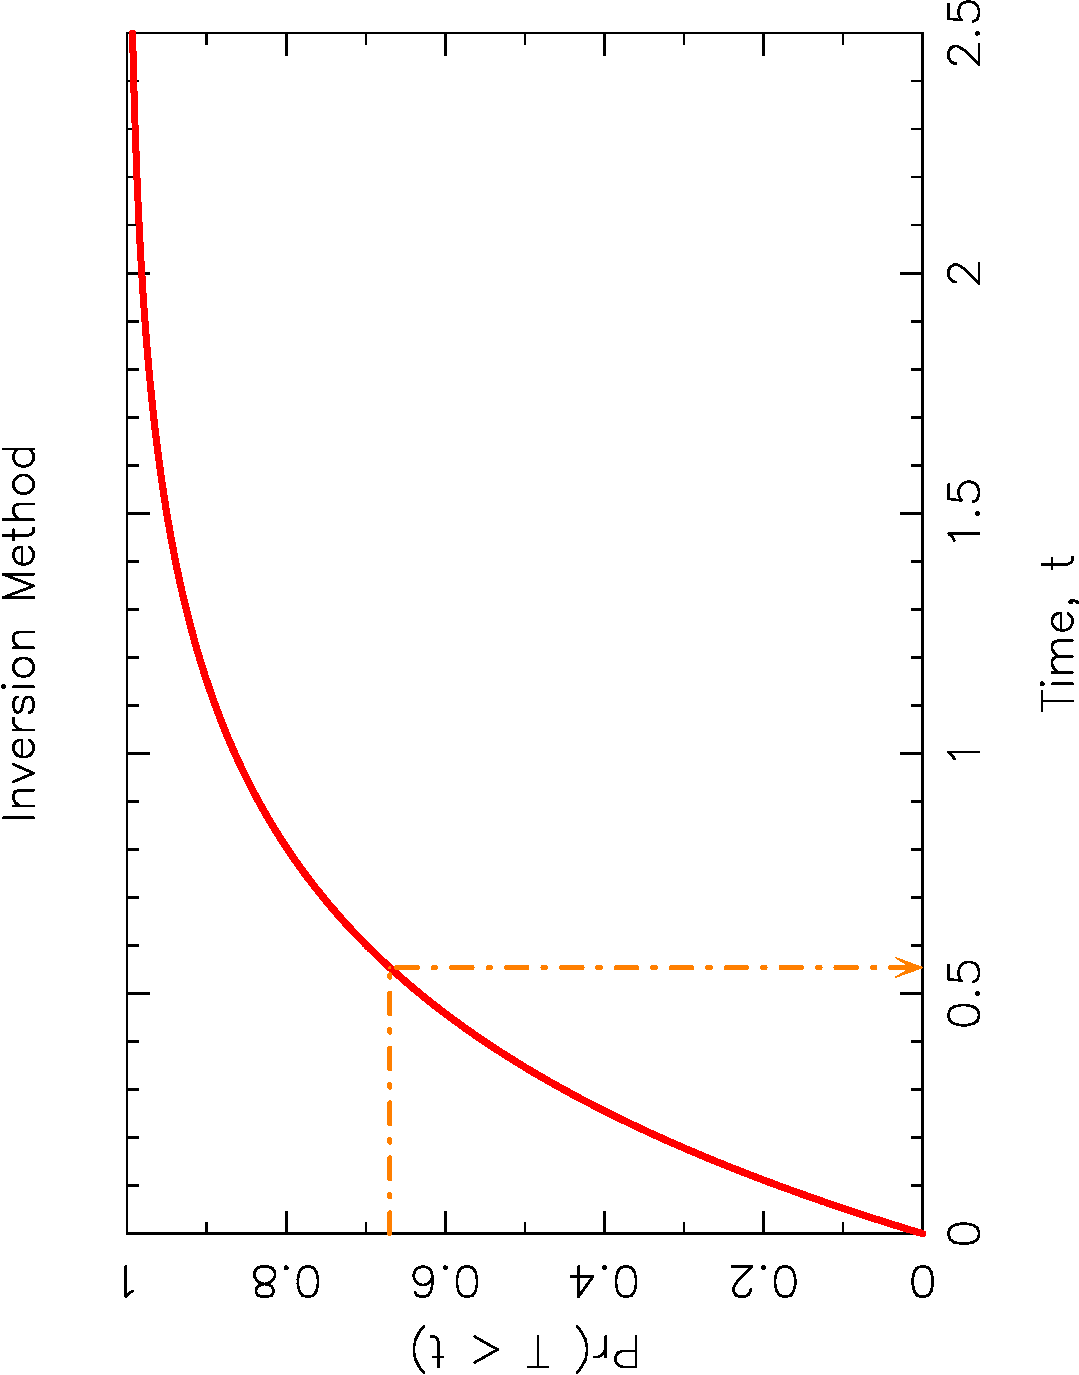
\includegraphics[width=0.6\textwidth,angle=270]{Inversion_Method}
	\caption[Inversion Method]{In order to sample a random variable following a given probability distribution, the inversion method is often used. One generates a uniformly distributed random number between 0 and 1, on the vertical axis, and looks for the corresponding value on the horizontal axis according to the cumulative probability distribution. Here, we have plotted the cumulative distribution function corresponding to an exponentially distributed random variable, $T$, with parameter $\lambda = 2.0$ ---see Eq (\ref{Exponential_Distribution}).}
	\label{Inversion_Method}
\end{figure}

Therefore, the Gillespie algorithm generating a stochastic realization of a Poissonian counting process (up to a maximum number of individuals), under which individuals arrive at an average rate $\lambda$ to a queue, can be summarized as follows:
\begin{enumerate}
	\item Initialize parameter $\lambda$
	\item Initialize a maximum number of individuals $M = 1000$
	\item Initialize the number of individuals in the queue as $n=0$.
	\item Initialize the time $t_0 = 0$
	\item Generate a random number $\Phi$ between 0 and 1. 
	\item Apply Eq (\ref{Random_Time}) to sample an inter-event time $t$. 
	\item Update queue $n \leftarrow n+1$. 
	\item Advance the time, this is, $t_n = t_{n-1} + t$
	\item If $n < M$, then go to 5 otherwise stop
\end{enumerate}
Then, the set $t_0, t_1, \dots, t_M$ is a single realization of the Poissonian counting process defining increasing stochastic times for the $M$ different arrivals.
\smallskip

A counting process is very simple. There is only one type of event that can happen: the arrival of a new individual. We already defined processes where, in addition, individuals can die or reproduce. In order to apply this algorithm, generally, to more complicated stochastic processes where different competing events may change the configuration of the system, we need to carefully understand the meaning of the total rate of something happening within the system. If something happens, it means there is an event that has occurred and, therefore, changed the system configuration. For example, for the Immigration-Death process conforming a \textit{sink} population (see section \ref{Immigration-Death-Process}), we have two different processes: immigrant arrivals and individual deaths. If we have $n$ individuals in the population, as we have discussed, the probability, in some little time $dt$, of a new individual arriving or one of the $n$ individuals dying will be the sum:
\begin{equation} 
\Pb[n \rightarrow n+1] + \Pb[n \rightarrow n-1] = \lambda\,dt + \mu \, n \,dt
\end{equation}
Therefore, the total temporal rate, $R(n)$, is:
\begin{equation} 
R(n) = \lambda + \mu \, n
\end{equation}
\smallskip

Notice the total rate $R(n)$ should account, exhaustively, for all the possible events that can ever happen in the system when it is in certain configuration, in this case, the population has $n$ individuals. While we are waiting for an event to happen, the total rate, $R(n)$, does not change at all, since $n$ is not changing. So, what is the probability that we are still waiting for an event to happen after certain time $t$? This should also be Poissonian because while we are waiting $R(n)$ is fully constant. Therefore, the probability that the system, at certain time $t$, is still waiting for an event to happen, this is, the probability that the next event happens at a time larger than $t$, this is, the time-to-next-event (or inter-event time), $T$, is larger than $t$ should be (see Eq (\ref{Eq_Exp_1})):
\begin{equation}
\Pb\{T>t\} =  e^{-R(n) t}
\end{equation}
and, again, it is crystal clear that:
\begin{equation}
\Pb\{T<t\} =  1 - e^{-R(n) t}
\end{equation}
which means that the time-to-next-event follows an exponential distribution with parameter the total rate $R(n)$. This is the most important point of the general Gillespie algorithm \citep{Gillespie76}. Notice that as the system changes configuration, the inter-event time still follows an exponential distribution but with a different parameter, the new total rate. In particular, imagine a system evolving to a frozen state when nothing else can happen, this is, the total rate of something happing in the system has exactly become zero. Therefore, if $R(n) = 0$, then $\Pb\{T<t\} = 0$ for any $t$ as large as you want, this is, the inter-event time becomes infinite because you can wait and wait but there is no further event to happen.  
\smallskip

Therefore, in order to sample inter-event times, we can safely follow the same strategy as before, this is, we can apply:
\begin{equation}
t     = -\frac{\log(\Phi)}{R(n)}
\label{Random_Time_General}
\end{equation}
but, once the time-to-the-next event has been determined, we should choose which particular event takes place. This should be done in proportion to the probabilities of each and every possible event. More precisely, Gillespie algorithm chooses an event by sampling the discrete probability distribution determined by the set of probabilities associated to each and every possible event in the system. For instance, in our example above, we should choose between either a new arrival or the death of one of the individuals in the system. So, we define two probabilities:
\begin{eqnarray}
p_1 &=& \frac{\lambda}{\lambda + \mu\,n} \nonumber \\
p_2 &=& \frac{\mu\,n}{\lambda + \mu\,n}  \label{p_1p_2}
\end{eqnarray}
and sample either the first (arrival) or the second (death) event accordingly. 
\smallskip

Although the Gillespie algorithm works for any one-step processes in continuous time, I will summarize now how to implement it for the \textit{sink} population above:
\begin{enumerate}
	\item Initialize parameters $\lambda$ and $\mu$. 
	\item Initialize a stopping criterion $t_M = 1000$
	\item Initialize the number of individuals in the system as $n=0$.
	\item Initialize the total number of events (or elemental steps) as $i=0$.
	\item Initialize the time $t_0 = 0$
	\item Generate a random number $\Phi$ between 0 and 1.
	\item Update total rate $R(n) = \lambda + \mu\,n$ 
	\item Apply Eq (\ref{Random_Time_General}) to sample an inter-event time $t$.
	\item Update $p_1$ and $p_2$ according to Eqs (\ref{p_1p_2}) 
	\item Sample\footnote{Statistical packages, such as $R$, implement functions to sample efficiently a discrete probability distribution given the set of probabilities associated to each possible event. This function is usually called $sample(\vec{p})$, where $\vec{p}$ is a $m$-dimensional probability vector and returns an index between 1 and $m$ to indicate the selected event.} a new event ($j$) to happen: $j \leftarrow sample(p_1, p_2)$ 
	\item If $j=1$ then update population $n \leftarrow n+1$ otherwise ($j=2$) $n \leftarrow n-1$
	\item Advance total number of steps $i \leftarrow i + 1$
	\item Advance the time, this is, $t_i = t_{i-1} + t$
	\item If $t_i < t_M$, then go to 6 otherwise stop
\end{enumerate}
This algorithm would yield a stochastic trajectory of a \textit{sink} population that increases due to random arrivals and decreases due to random individual deaths until time is greater than $t_M$, this is, it follows an immigration-death process (see section \ref{Immigration-Death-Process}). For more complicated processes, it will be essential to write down an exhaustive table of all possible events with their associated probability rates. In general, for a system whose configuration is defined by a state vector $\vec{n}$, where there are $m$ possible events, we can sketch such a table as:
\begin{center}
	\begin{tabular}{lc}
		\textbf{Event} & \textbf{Event Rate} \\
		
		1          & $R_1(\vec{n})$ \\
		2          & $R_2(\vec{n})$ \\
		$\dots$    & $\dots$        \\
		$m$        & $R_m(\vec{n})$ \\
		           &                \\
		\textbf{Total Rate} & $R(\vec{n}) = \sum_{i=1}^m R_i(\vec{n})$
	\end{tabular}
\end{center}

\subsection{The Immigration-Birth-Death Process: Two Populations}
As an example, let us now write an events table for an immigration-birth-death process of two populations of two different species colonizing the same island. The state of such a system is defined by a two-dimensional state vector, $\vec{n} = (n_1, n_2)$, where $n_1$ and $n_2$ are the number of individuals of the first and second species, respectively. Each species colonizes the island at a species-specific rate ($\lambda_i$, for $i=1,2$), and individuals die and reproduce at species-specific rates ($\mu_i$, for $i=1,2$ $\beta_i$, for $i=1,2$) as well. There are then six possible events, which are summarized in the following events table with their rates:

\begin{center}
	\begin{tabular}{lcc}
		\textbf{Event} & \textbf{Configuration Change} & \textbf{Event Rate}                                                               \\
		
		1      & $n_1 \rightarrow n_1 + 1$ & $R_1(\vec{n}) = \lambda_1$              \\
		2      & $n_1 \rightarrow n_1 + 1$ & $R_2(\vec{n}) = \beta_1\,n_1$           \\
		3      & $n_1 \rightarrow n_1 - 1$ & $R_3(\vec{n}) = \mu_1\,n_1$             \\
		4      & $n_2 \rightarrow n_2 + 1$ & $R_4(\vec{n}) = \lambda_2$              \\
		5      & $n_2 \rightarrow n_2 + 1$ & $R_5(\vec{n}) = \beta_2\,n_2$           \\
		6      & $n_2 \rightarrow n_2 - 1$ & $R_6(\vec{n}) = \mu_2\,n_2$             \\
		       &                           &                                         \\
		       & \textbf{Total Rate}       & $R(\vec{n}) = \sum_{i=1}^6 R_i(\vec{n})$
	\end{tabular}
\end{center}
We can then use the Gillespie algorithm above to generate a stochastic trajectory of the system. All we need is to define the total rate as a sum over the 6 event rates. We also require to define a corresponding 6-dimensional probability vector, $\vec{p}$, again by dividing each event rate by the total rate. Finally, we require to sample this discrete probability distribution to choose an specific event to occur, and update the configuration of the system accordingly (see corresponding configuration change in the table above).  
\smallskip

This example corresponds to two species independently colonizing an island. It is then a two-dimensional one-step stochastic process. The Gillespie algorithm is powerful and simple. It can be easily generalized to more dimensions and even species interactions \citep{Sole02}. All that is required is, first, the characterization of the state of the system with a suitable (multi-dimensional) state variable that fully defines the configuration of the system, and, second, the exhaustive calculation of all transition events that can possibly occur between all different system configurations and their corresponding probability rates.  

\section{Models and Data: the Likelihood Approach}
According to our view, natural systems evolve stochastically jumping from a given configuration to another at specific rates. Imagine we measure a system to record its configuration every month. After a while, we can say our system has visited a given series of configurations along time. Some jumps or transitions will be frequent. Others will be very rare. Others will be forbidden. Can this time series of measured configurations reveal information about the underlying processes driving the dynamics of the system? The likelihood concept allows to address this interesting question. We will review here this concept again through a simple example.
\smallskip

Imagine you have a front desk with $M$ attendants. Customers arrive and line up in front of each attendant. Assuming there are no people in front of any attendant at the initial time, $t_0 = 0$, imagine you measure the number of customers in front of each attendant after a given time $t$. You end up with a series of measures, $n_1, \dots, n_M$, where $n_i$ is the number of people in front of the $i$-th attendant. Does each of these lines conform to a Poissonian counting process? If we assume the answer is yes, what is the best estimate of the common rate, $\lambda$, driving the Poissonian dynamics of each line independently? Let us assume that each line is governed by an independent Poissonian process of rate $\lambda$. Then, we can exactly calculate the probability of obtaining the series of measures we have obtained, $n_1, \dots, n_M$, after a time $t$:
\begin{equation}
\Pb\{n_1, \dots, n_M\} =  \frac{(\lambda\,t)^{n_1}}{n_1!}e^{-\lambda t}\dots  \frac{(\lambda\,t)^{n_M}}{n_M!}e^{-\lambda t}
\end{equation}

This probability depends on the empirical data, $n_1, \dots, n_M$, and the time $t$ at which the empirical data are obtained, and an unknown parameter, $\lambda$. Let us write down this dependency explicitly, and arrange: 
\begin{equation}
\Pb\{n_1, \dots, n_M | \lambda\} =  \frac{(\lambda\,t)^{n_1+\dots+n_M}}{n_1!\dots n_M!}e^{-M \lambda t}
\label{Lk1}
\end{equation}

Therefore, under the hypothesis of independent Poissonian counting process described by the same rate $\lambda$, our observed series, $n_1, \dots, n_M$, has an associated probability, which cannot be calculated because the model parameter $\lambda$ is unknown. This probabality is often called the likelihood of the data given, in this case, independent paral.lel Poisson processes of parameter $\lambda$. Since $\lambda$ is unkown, we may ask which value of $\lambda$ maximizes this probability. This optimal $\lambda$ is commonly called the maximum likelihood estimate of the model parameter. If you think carefully about it, this maximum likelihood estimate is the most reasonable choice for parameter $\lambda$. As said, the last probability (Eq (\ref{Lk1})), regarded as a function of the model parameter $\lambda$, is called the likelihood function for the data at hand:
\begin{equation}
F(\lambda |n_1, \dots, n_M;  t) =  \frac{(\lambda\,t)^{n_1+\dots+n_M}}{n_1!\dots n_M!}e^{-M \lambda t}
\label{Lk2}
\end{equation}

In what follows, since our data, $n_1, \dots, n_M$ at time $t$, once measured, remain constant, for simplicity, we will note our likelihood as a only function of $\lambda$, $F(\lambda)$, dropping any dependency on our data. Interestingly, the optimal $\lambda$ that maximizes $F(\lambda)$ can be calculated by looking for the value of $\lambda$ that makes the first derivative of $F(\lambda)$ equal to zero. However, we build first the logarithm of the likelihood function\footnote{Since the logarithm is a monotonic increasing function, the functions $F(\lambda)$ and  $H(\lambda)$ have their maxima for the same value of $\lambda$.}, the logLikelihood function, $H(\lambda) = \log(F(\lambda))$, because it is easier to derive:
\begin{align}
H(\lambda) &= -M\,\lambda\,t + (n_1+\dots+n_M)\,\log(\lambda\,t) - log(n_1!\dots n_M!)\nonumber\\
\frac{dH}{d\lambda} &= -M\,t + (n_1+\dots+n_M)\frac{1}{\lambda} = 0                      \nonumber\\
\lambda &= \frac{n_1+\dots+n_M}{M\,t} \label{MLE}
\end{align}

Therefore, in words, according to Eq (\ref{MLE}), the maximum likelihood estimate of $\lambda$\footnote{You can check that this extreme value is a maximum in the usual way, this is, by taking the 2nd derivative of $F(\lambda)$, and checking that it is negative when evaluated at this value.} is the average of the number of customers over the $M$ different counters divided by the time span $t$ during which they have arrived.

\subsection{Colonization and extinction processes in an island}
In this example, we highlight another important point in modeling natural systems. We require first to decide which potentially measurable variables we will use to carefully characterize the state of the system under study. This depends on the which particular question we want to addres, but, in all cases, it is the first crucial decision we should make. In most previous applications, we have chosen to describe the system by the number of individuals, this is, our state variable, $N$, can take all non-negative integer values. However, for some applications, it is useful to coarse-grain this description. Sometimes it is difficult to measure accurately the number of individuals of a species. In a given island, natural reserve or particular site, it is often easier to assess whether the species is present or absent. In this case, the variable characterizing the system can only take two values to indicate either presence or absence of the species under study. This {\it coarse-grained} variable will be a Boolean stochastic variable, $X$. Conventionally, we will say it will take the value 1 if the species is present, and 0, if it is absent. Therefore, the system now can only be in two different states (0 and 1). What are then the processes by which the system jump between these two possible configurations?  These two configurations may change as a result of two ecological processes: species extinction ($1 \rightarrow 0$), and species colonization ($0 \rightarrow 1$). 
\smallskip

If we know how to describe a system by enumerating all its possible configurations and what are the events (and their associated rates) allowing the system to jump between configurations, then we can apply the Gillespie algorithm to generate stochastic replicates, and we can write down ---and tried to solve--- the master equation describing the temporal evolution of the discrete probability distribution over configurations.
\smallskip

Therefore, in modeling a colonization-extinction process of a species in an island, we need to make an assumption about the rates at which these two processes occur. The simplest assumption is (compare to Eq (\ref{eq:pb})):
\begin{eqnarray}
\Pb\{ 0 \longrightarrow 1 \} & = & c\,dt \nonumber\\
\Pb\{ 1 \longrightarrow 0 \} & = & e\,dt
\label{eq:c-e}
\end{eqnarray}
The inverse of $c$ is a measure of the average time the system is empty until the focal species colonizes the island. Analogously, one over $e$ is the average time it takes for the species to go extinct. We make the assumption that these rates remain constant in time. 
\smallskip

Now we are in a position to write down the master equation describing the temporal evolution of the discrete probability distribution associated to the presence-absence stochastic variable. As any other Boolean stochastic variable, this probability distribution is just characterized by two values: probability of presence ($P_1$) and probablity of absence ($P_0$). The full master equation is given by:
\begin{eqnarray}
\frac{dP(0,t)}{dt} &=&    e\, P(1,t) \,\, - \,\, c\, P(0,t)  \nonumber \\
\frac{dP(1,t)}{dt} &=&    c\, P(0,t) \,\, - \,\, e\, P(1,t)  
\label{me_c-e}
\end{eqnarray}
where $P(0,t) \equiv P_0$ and $P(1,t) \equiv P_1$. When a system can just visit a finite number of configurations, the master equation has always a matrix representation: 
\begin{equation}
\label{me_matrix}
\frac{d}{dt}\left(
\begin{array}{c}
P_0 \\ 
P_1 
\end{array}
\right) = \left[\begin{array}{cc}
-c &  e \\
 c & -e 
 \end{array} 
\right]
\left(
\begin{array}{c}
P_0 \\ 
P_1 
\end{array}
\right)
\end{equation}

As you see, Eqs (\ref{me_c-e}) ---or in matrix form, Eq (\ref{me_matrix})--- is nothing but a particular case of Eqs (\ref{me_1}) for a the system that can only be in two alternative configurations. Since $P_0$ and $P_1$ are complementary probabilities, they must sum up to one. Therefore, the temporal evolution of the probability distribution is determined by just one equation. Conventionally, we use the equation for the probability of the species being present at time $t$, which is called occupancy probability:
\begin{equation}
\frac{dp}{dt} = c\,(1-p) - e\,p
\label{eq:HANSKI01}
\end{equation}
where $p$ has been defined as $P_1$. For instance, if we observe that the species is absent at time zero, $p(0) = P_1(0) = P(1,0) = 0$, then the solution for the species occupancy probability at time $t$ reads:
\begin{equation}
\label{t_10}
p(t) = \frac{c}{e+c} ( 1 - \exp(-(e+c)t ))
\end{equation}
This solution\footnote{In order to solve ODE (\ref{eq:HANSKI01}), we use the method of variation of parameters, just as we did to find the solution of ODE (\ref{Eq_n_1}).} is the probability of a species being present in the island after some time $t$, given that the species was initially absent. 
\smallskip

When a system can just visit a finite number of configurations, we can always write down a discrete-time representation of the master equation, Eq (\ref{me_matrix}). This discretization adds one extra model parameter, which is the time between observations, $\Delta t$:
\begin{equation}
\label{Markov_model}
\left(
\begin{array}{c}
P_0 \\ 
P_1
\end{array}
\right)_{t+\Delta t} = \left[\begin{array}{cc}
T_{00} & T_{01} \\
T_{10} & T_{11}
\end{array} 
\right]
\left(
\begin{array}{c}
P_0 \\ 
P_1 
\end{array}
\right)_{t},
\end{equation}
where $T_{10}$ ($T_{01}$) is the probability of (not) finding certain species at time $t$ given that it was absent (present) at time $t=0$. In addition, conditional probabilities $T_{00}$ and $T_{11}$ satisfy $T_{00}=1-T_{10}$ and $T_{11}=1-T_{01}$, respectively. Discrete-time stochastic models, such as the one given by Eq. (\ref{Markov_model}), are usually called Markov chain models. In Markovian models, the state of the system after some time $\Delta t$ depends only on the state of the system at time $t$ and a given transition matrix, whose elements are transitions probabilities. In our case, we can consistently derive all four entries of the transition matrix in terms of the colonization and extinction rates, $c$ and $e$ (see Eq. \eqref{t_10}):
\begin{equation}
\label{T_00}
\left\{
\begin{array}{ccc}      
T_{10}(\Delta t| c, e) &=&  \frac{c}{e+c} ( 1 - \exp(-(e+c)\Delta t) )\\  
T_{01}(\Delta t| c, e) &=&  \frac{e}{e+c} ( 1 - \exp(-(e+c)\Delta t) )\\
\end{array}
\right.
\end{equation} 
To sum up, the stochastic discrete-time version of the model ---see Eq (\ref{Markov_model})--- gives the temporal evolution of the probability distribution, $(P_0,\, P_1)$, over discrete time steps, $\Delta t$. This parameter is usually chosen to be 1 in suitable time units (one week, one month, etc). 
\bigskip

As we have seen in our previous example, the central point in likelihood estimation is the ability to calculate the probability of observing a set of data under given model assumptions and parameter values. We have written the discrete model given by Eq (\ref{Markov_model}) because data are always obtained at discrete time values. Assume we are given a data vector whose elements represent island configurations at increasing (not necessarily equally-spaced) time values, $t_1, \dots, t_N$:
\begin{equation}
	\label{eq:data}
	M = 
	\left[
	\begin{array}{rccccccc}
	& t_1 & t_2 & t_3 & t_4  & t_5 & \dots & t_N                             \\
	& 1 & 0 & 1 & 1 & 1 & \cdots & 0                                   \\
%	2:    & 1 & 1 & 1 & 0 & 1 & \cdots & 1                                     \\
%	\vdots\phantom{::} & \vdots & \vdots & \vdots & \vdots & \vdots &  & \vdots \\
%	S_P:  & 0 & 1 & 0 & 1 & 1 & \cdots & 0                                    \\
	\end{array}
	\right],
\end{equation}
\smallskip

If we assume that the data above have been generated by random colonization-extinction processes of a given species characterized by the colonization extinction rates $(c,\, e)$ , it is easy to calculate the likelihood of observing a series of occupancies across time, for instance, the vector $(1, 0, 1, 1, 1, \cdots, 0)$. If we generally write a presence/absence vector as ${\boldsymbol n}=(n(t_1),\dots,n(t_N))$ from times $t_{1}$ to $t_N$, then the probability of observing a given temporal presence/absence sequence, ${\boldsymbol n}$, is \citep{Alonso2015}:
\begin{equation}
P( {\boldsymbol n} | c, e) = \prod_{j=1}^{N-1}T_{n(t_{j+1}),n(t_j)}(t_{j+1}-t_{j}| c,e) 
\label{Eq_lk}
\end{equation}

The last equation can be regarded as a likelihood function depending only on two model parameters, $(c,\,e)$. Again, given an observed series of occupancies for a species across time, we can ask for the values of $c$ and $e$ that maximize the likelihood of making exactly that series of observations. Usually, the search for optimal values in multi-parametric functions, such as Eq (\ref{Eq_lk}), is done by using appropriate numerical methods.
\smallskip

However, when an island has been sampled at regular times, the two independent matrix entries, $T_{10}$, and $T_{01}$, i.e., respectively, the colonization and extinction transition probabilities, can be estimated simply, by counting the frequency of observed transitions: 
\begin{eqnarray}
\label{N_10}
T_{10} & = & \frac{N_{10}}{N_{10} + N_{00}} \\
\label{N_01}
T_{01} & = & \frac{N_{01}}{N_{01} + N_{11}}
\end{eqnarray}
where $N_{10}$ is the number of times a transition to colonization has been observed, $N_{01}$ is the number of times a transition to extinction has occurred, $N_{00}$ is the number of times a species has remained absent from the system, and $N_{11}$ is the number of times a species has remained present in the island from a given observation to the next. Provided regular sampling times, $\Delta t$,  one can show that these are the maximum likelihood estimates (m.l.e.) of the entries of the stochastic transition matrix, $T_{10}$ and $T_{01}$\footnote{In order to demonstrate that this is so, we require first to particularize the likelihood function Eq (\ref{Eq_lk}) for a constant $\Delta t$ between time observations, and derive the resulting function with respect to both $T_{10}$ and $T_{01}$ and equal both derivatives to zero. If you solve the system for the two unknowns, $T_{10}$ and $T_{01}$, you will see that the values that maximize this function are given by Eqs (\ref{N_01})-(\ref{N_10}).}. Once the maximum likelihood estimates of these transition probabilities have been found, we can invert equations Eqs (\ref{T_00}) to determined the maximum likelihood estimates of the initial model parameters $(c,\, e)$:
\begin{equation}
\begin{array}{ccccc}
\frac{e}{c} &=& \frac{T_{01}}{T_{10}}           &=&      \frac{N_{01}(N_{10}+N_{00})}{N_{10}(N_{01}+N_{11})}\\
e + c       &=& -\frac{1}{\Delta t}\log(1 - (T_{01}+T_{10})) &=& -\frac{1}{\Delta t}\log\left(\frac{N_{00}N_{11}-N_{01}N_{10}}{(N_{10}+N_{00})(N_{01}+N_{11})}\right)
\end{array}
\end{equation}

\newpage
\bibliographystyle{mee}
\bibliography{ecology_david}  % The file containing the bibliography


\newpage
\setcounter{section}{0}
\renewcommand{\thesection}{P\arabic{section}}

\section{Practicum}
An open metapopulation is a system of $N$ patches that can be occupied or not by a species of interest. The species in a patch can undergo extinction at rate $\delta$. Local colonization is controled by the rate $\beta$, and depends on the global density of patches $n/N$, where $n$ is the number of occupied patches, and empty patches can be also colonized through external immigration events, at rate $\mu$. Show that the average, over Gillespie-generated stochastic trajectories, for the number of occupied patches from an open metapopulation of $N$ patches follows the deterministic equation: 
\begin{equation}
\frac{dX}{dt} = \beta\,\left(1-\frac{X}{N}\right)\,X + \mu\,(N-X) - \delta\, X
\end{equation}
where $X$ is the average number of occupied patches at time $t$, this is, $\langle n \rangle$. 

\begin{enumerate}
	\item Take first the determistic equation, find stationary points and study their stability.	
	\item Solve this ODE numerically using at least two different numerical method. The initial condition is given by the absence of occupied patches at time $t_0 = 0$. This will yield a function $N(t)$. 
	\item Build 100 stochastic simulations starting (all of them) with no occupied patches at time $t_0 = 0$ using the Gillespie algorithm described in page 13. Sample the number of individuals at increasing time intervals for 100 different times. Choose an appropriate constant time between samplings, $\Delta t$. Therefore, sampling times will be defined as $t_i = i\,\Delta t$ for $i=0$ to $i=100$.   
	\item Plot 5 stochastic trajectories between $t_0=0$ and $t_{100} = 100\,\Delta t$ and the function $N(t)$ derived in step 1. 
	\item Plot the average of number of individuals over the whole 100 stochastic simulations along with the deterministic function found at point 1, $N(t)$. 
	\item Try this for different parameter choices. 
\end{enumerate}


\section{Practicum}
Show that the average for the number of individuals in an island over Gillespie-generated stochastic trajectories following an immigration-death model with parameters $\lambda=10$ and $\mu = 2$ (see section \ref{Immigration-Death-Process}) accurately approximates the deterministic temporal evolution for the number of individuals on the island. Please follow the following steps:
\begin{enumerate}
	\item Take first the determistic equation:
	\begin{equation}
	\frac{dN}{dt} = \lambda - \mu N
	\end{equation} 
	Solve this ODE using the method of variation of parameters when the initial condition is given by the absence of individuals at time $t_0 = 0$. Alternatively, you can also use numerical integration to solve this ODE. In any case, this will yield a function $N(t)$. 
	\item Build 100 stochastic simulations starting (all of them) with no individuals at time $t_0 = 0$ using the Gillespie algorithm described in page 13. Sample the number of individuals at increasing 100 times. Choose an appropriate constant time between samplings, $\Delta t$. Therefore, sampling times will be $t_i = i\,\Delta t$ for $i=0$ to $i=100$.   
	\item Plot 5 stochastic trajectories between $t_0=0$ and $t_{100} = 100\,\Delta t$ and the function $N(t)$ derived in step 1. 
	\item Plot the average of number of individuals over the whole 100 stochastic simulations along with the deterministic function found at step 1, $N(t)$. 
\end{enumerate}
 
\newpage
\setcounter{section}{0}
\renewcommand{\thesection}{E\arabic{section}}

\section{First Question for the Exam}
Show that the probability generating function of a Binomial random variable is given by:
\begin{equation}
	G(x) = (p\,x + 1-p)^N
\end{equation}
where $p$ and $N$ are the two parameters of the Binomial probability distribution. 
\smallskip

From the expression of the probability generating function above, calculate the expected value and the variance of a Binomial random variable. 

\section{Second Question for the Exam}
There is a crazy researcher making measurements to determine the rate at which customers line up in front of a front-desk. He has made measurements for a period of time, which are summarized in the following data:
\begin{equation}
\label{eq:Measures}
{\bf D} = 
\left[
\begin{array}{rccccccc}
& t_1 & t_2 & t_3 & t_4  & t_5 & t_6 & t_7                             \\
& 0   & 3   & 5   & 8    & 12  & 14  & 18                               
\end{array}
\right]
\end{equation}
where the 2nd row represents number of individuals, and the times of the observations (in minuts) are given by $(t_1, t_2, t_3, t_4, t_5, t_6, t_7) = (0, 10, 17, 26, 33, 40, 50)$. Assuming the queue follows a Poissonian counting process, what is the maximum likelihood estimate for the constant rate, $\lambda$, characterizing this process? 

\section{First Question for the Exam (Bis)}
Use the probability generating function of a Poissonian counting process (of rate $\lambda$) to show that such a process has both average and variance increasing with time at the same rate $\lambda$. 

\section{Second Question for the Exam (Bis)}
In 1967, MacArthur \& Wilson published a book ``The Theory of Island Biogeography'' (TIB) to explain the factors controling species diversity on {\em islands} at certain distance from the continent, the {\em mainland}. Some crazy researchers are trying to expand that theory, which considers only the processes of colonization and extinction (see Eqs (\ref{eq:c-e}) in my notes), to consider also the presence of species in the lake sediment. Lakes are natural islands. These crazy researchers start considering only one  unicellular algae species. This species can arrive to the lake through colonization (\textit{colonization process}), and go fully extinct (\textit{extinction process}), but, in addition, it can also produce dormant eggs that sediment into the lake bottom (\textit{sedimentation process}). Therefore, species can be fully absent from the water and sediment, be only in the water, be only in the sediment, or be both in water and sediment. Of course, the algae cannot colonize directly the sediment without being present first in the water column and producing dormant eggs. Use the following model parameters: $\mu_1$ as the species extinction rate from the water column, $\mu_2$ as the species extinction rate from the sediment, $c_1$ as the species colonization rate into the water column from outside, $c_2$ as the re-colonization rate of the water column from the sediment, and $\sigma$ as the species sedimentation rate (or rate of species arrival into the sediment through production of dormant eggs). Please answer: 

\begin{enumerate}
	\item How could you describe the configuration of the system in these four different states and all possible transitions (and their rates) between them? (hint: use a graph where the nodes are the different configurations and the edges the possible transitions between them).
	\item Since the system can only be in four different configurations, the master equation will be a system of 4 coupled ODEs. Can you write it in matrix form (see Eq. (\ref{me_matrix}) in my notes)?    
	\item Can you calculate the probability distribution describing the stationary state? (hint: this discrete probability distribution has only 4 different probabilities).
\end{enumerate}

\end{document}
